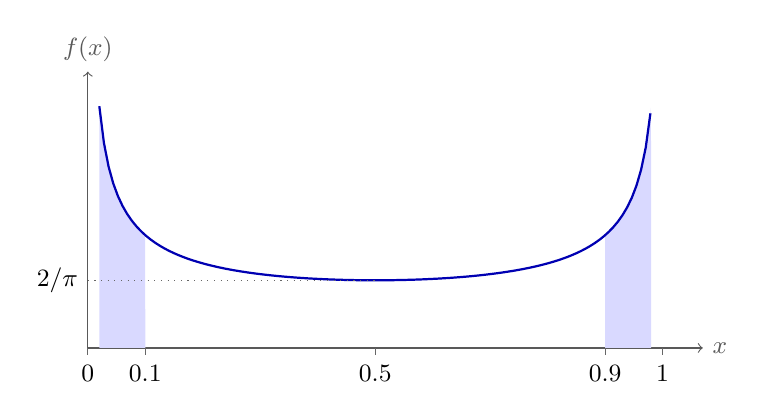
\begin{tikzpicture}[x=7.3cm,y=1.35cm]
\draw[->,black!65] (0,0)--(1.07,0) node[right,font=\small] {$x$};
\draw[->,black!65] (0,0)--(0,2.6) node[above,font=\small] {$f(x)$};
\fill[blue!15] (0.02,0)--plot[domain=0.02:0.1,samples=40] (\x,{1/(pi*sqrt(\x*(1-\x)))})--(0.1,0)--cycle;
\fill[blue!15] (0.9,0)--plot[domain=0.9:0.98,samples=40] (\x,{1/(pi*sqrt(\x*(1-\x)))})--(0.98,0)--cycle;
\draw[blue!70!black,thick] plot[domain=0.02:0.98,samples=120] (\x,{1/(pi*sqrt(\x*(1-\x)))});
\foreach \x/\lab in {0/0,0.1/0.1,0.5/0.5,0.9/0.9,1/1}{
  \draw[black!60] (\x,0)--(\x,-0.07);
  \node[below,font=\small] at (\x,-0.07) {$\lab$};
}
\draw[dotted,black!60] (0,0.63662)--(0.5,0.63662);
\node[left,font=\small] at (0,0.63662) {$2/\pi$};
\end{tikzpicture}
